\chapter{Developer and User Documentation}

During the study thesis detailed documentation and tutorials for the \osmvt{} project has been created. The documentation was separated into a user-centric and developer-centric part.
All of this information was provided on the project website (\url{http://osm2vectortiles.org}). However when the project was publicly released and people started to get interested in the project, two main problems occurred:

\begin{itemize}
    \item The tutorials targeted at regular users were too complicated and error prone
    \item Developers want to have the documentation on GitHub right next to the code and not on the project website
\end{itemize}

With this knowledge it was decided to move the developer-centric documentation into README files right next to the code and simplify the user-centric tutorials to eliminate most beginner errors.

\begin{figure}[H]
  \centering
  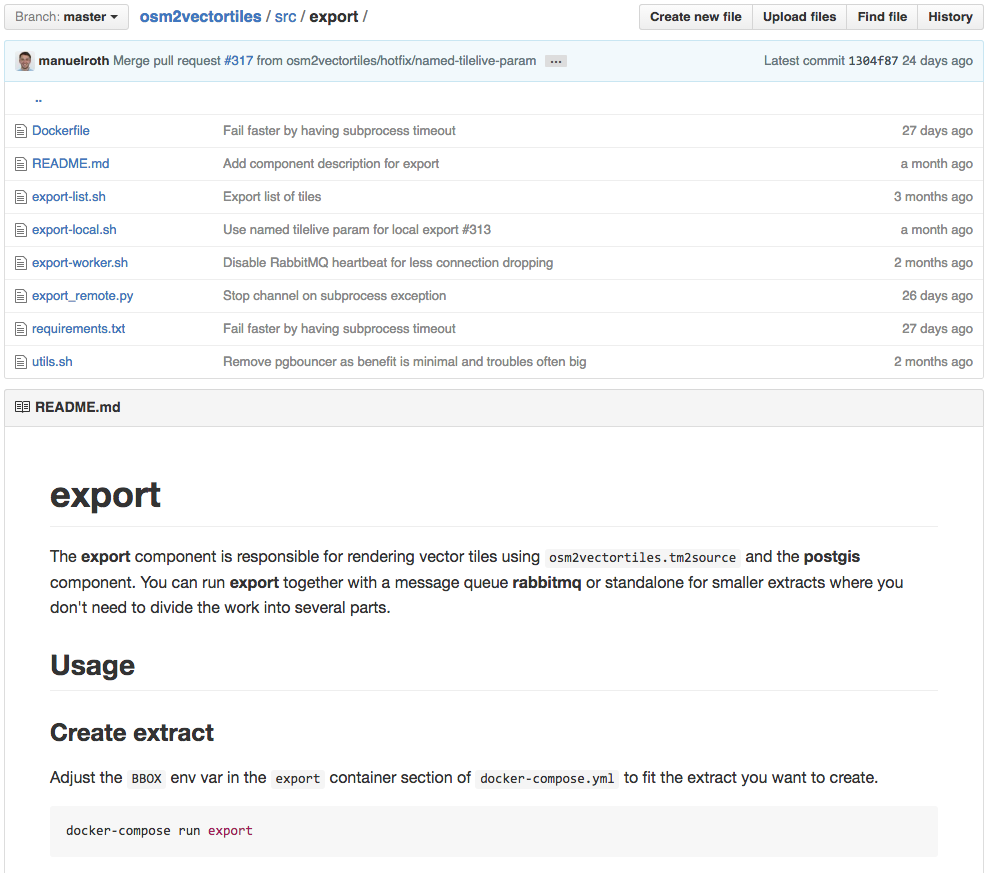
\includegraphics[width=1.0\textwidth]{images/documentation/developer_documentation}
  \caption{Documentation of the export component using a README file}
  \label{developer_documentation}
\end{figure}

\autoref{developer_documentation} and \autoref{user_documentation} show the documentation in the repository on GitHub and on the project website. The documentation can be found either on GitHub (\url{https://github.com/osm2vectortiles/osm2vectortiles}) or on the project website (\url{http://osm2vectortiles.org}).

\begin{figure}[H]
  \centering
  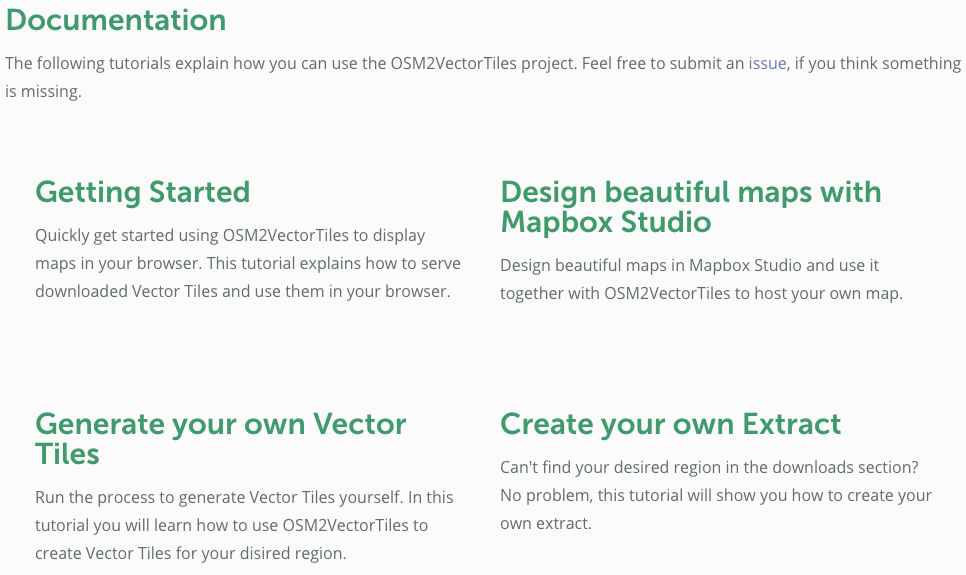
\includegraphics[width=1.0\textwidth]{images/documentation/user_documentation}
  \caption{Simplified overview of user documentation on the project website}
  \label{user_documentation}
\end{figure}